\documentclass[dvipdfmx]{jreport}
% Use the lineno option to display guide line numbers if required.

%\usepackage[]{graphicx}
\usepackage[]{listings}
\setcounter{secnumdepth}{4}

\usepackage[margin=20truemm]{geometry}
\usepackage{minted}
\usepackage[dvipsnames]{xcolor}   
\usepackage{fontawesome}
\usepackage{xspace}
\usepackage{chartdef}
\usepackage{comment}
\usepackage{subfiles}
\usepackage{bm}
%\usepackage{easy-todo}
\usemintedstyle{solarized-light}
\setminted[shell]{breaklines=true}

%\usepackage{easy-todo} % todo list
\usepackage[japanese]{minitoc} % table of contents in chapter
\usepackage{siunitx} % tabular and si unit?
\usepackage{fancyreport}
\usepackage{tocloft} % avoid overlap of chapter number and its title
\usepackage{hyperref}
\renewcommand\cftchapnumwidth{9ex}
\newcommand{\target}{g4simcat}
\newcommand{\taskdone}{\vspace{5pt}\noindent\textcolor{ForestGreen}{\faCheckCircleO}\xspace}
\newcommand{\taskdoing}{\vspace*{5pt}\noindent\textcolor{BurntOrange}{\faArrowCircleORight}\xspace}
\newcommand{\taskinit}{\vspace*{5pt}\noindent\textcolor{BrickRed}{\faPencilSquareO}\xspace}




\title{Cosmic-ray PNT using air shower front}

% Use letters for affiliations, numbers to show equal authorship (if applicable) and to indicate the corresponding author
\author{大田 晋輔 \\ 大阪大学 核物理研究センター}


\begin{document}
%%% minitoc
\dominitoc
%%%

\maketitle

% 目次の出力
\tableofcontents

\listoftodos
\clearpage
\chapter{本論}

\section{Introduction}

% several technics of PNT without GNSS

Techniques for positioning, navigation, and timing are obviously crucial not only for our personal daily life but also for the imaging of huge materials (火山の透視), automated industry, and so on. The PNT using the radio wave from the satellite, {\it e.g.} GNSS is widely used technique, however, the performance is strongly degraded if the radio waves are blocked by the obstacles such as the buildings, soils, and sea water. To overcome this problems, indoor PNT techniques are developed using the electric waves from the references such as WiFi station, laser, ... But there are different kind of obstacles may exist indoor environments or the electric waves cannot penetrate the soils nor the sea water. The application of cosmic-ray muon instead of the electric waves is performed to realize the imaging of large  objects, timing synchronization, and navigation. The muonic position system (muPS) and Muometric Wireless Navigation System  (MuWNS) was proposed by Takana based on the several time-of-flight measurements between the clients and some reference detectors assuming the velocity of the muon is the same as the speed of lights. In this method due to the clock drifting the positioning less than a few meter accuracy cannot be achieved since the frequency of the muon coincidence measurement is limited. Tanaka proposed a new concept of Vector muPS, where the angle of muon is measured by the reference and the position of the receiver is estimated by combining the angle and position measured by the reference detector. But Vector muPS does not provides the timing synchronization. 

Here we propose the new concept using the air shower where the cosmic-ray muon belongs to, toward the simultaneous positioning and timing synchronization using the cosmic-ray muon. The air showers are constantly pouring down on the ground.
The time evolution of the air showers can be estimated by measuring the shower front which travels with the speed of light. Assuming the muon is travels along the normal direction of the shower front, the virtual reference detector can be positioned at any place inside the shower front. The shower front is known to have a certain thickness for example, 100 ns at xxx m front the shower center with xxx-eV primary cosmic ray \todoi{大気シャワーの厚さについての文献を入れる}

If the detection frequency is much larger than the muon \todoi{大気シャワーフロント情報同定のエネルギー依存性の導出}, the uncertainly in the PNT can be compensated according to the statistics. For example, the frequency of coincidence with shower and muon is 10000 per second, the resolution becomes order of ten centimeter. In this paper, the efficiency of the shower front measurement and the performance of positioning and time synchronization with air-shower virtual reference are described.



% 文字数は Latex workshop の count words を使えばカウントできる

\chapter{執筆計画}

\section{執筆にむけて}

アメリカではすでに大統領がサインするなどミュオンを用いた測位システムは注目を浴びている。また、アルメニアなど海外では新しいアイデアが出てきているので、我々のアイデアを形にして国際的に早急に提示する必要がある。

2024年9月2日に開催されたシンポジウムでは、オープンセッションの発表に対して、KEKの下村さんが画期的なアイデアであるということをお伝えくださり、講評でも KEK の三宅さんが、よくわからないけれど斬新なアイデアであり、歓迎されるものであるという内容の話をしていただけた。懇親会の会場においても非公式ながら期待を寄せる言葉をいただいたし、スーパーバイザーとなる（懇親会でそういう話をきいた）総合科学研究機構の杉山さんからも帰り道で質問を受けた。

日本発の技術となるように頑張ってほしいという言葉もあるし、自分自身もこれは私の成果であるとなるように早急にアイデアをまとめる。

\section{日程}

完全に決まったわけではないが、現時点では2ヶ月程度で、概念設計をおこなって特定のシステムに対する性能を提示するような論文を執筆することを目標とする。そのためのシミュレーションおよび執筆に2ヶ月をあてて、のこり1ヶ月で投稿することを目標にする。

\begin{table}[h]
   \centering
   \caption{執筆スケジュール}
   
   \begin{tabular}[t]{cl}
      \hline
      \hline
      2024/09/02 & シミュレーションおよび執筆開始 \\   
      2024/10/31 & 初稿完成、回覧開始 \\
      2024/11/15 & 回覧終了、投稿準備 \\
      2024/11/20 & 投稿 \\
      \hline
      \hline
   \end{tabular}
\end{table}

\section{論文の内容}
研究は開始されたばかりであり、ユースケースのすべてを覆うことができるわけではないため、たくさんのことがかけるわけではない。しかし、特許申請につながるような論文の公表をする必要があると考えている。まずは尖った内容のシミュレーションを終えて、それについてまとめるところから始める。

ポイントは大気シャワーのシャワーフロントの時間発展が時刻同期・測位にどのような影響を与えるかということになる。まずはシャワー面が理想的なシャワー面である場合のシミュレーションを行って、性能を推定することから始める。

\subsection*{背景}
\begin{itemize}
   \item なぜ衛星を使わないPNTが必要であるのか？衛星が使えない場所でのPNTが必要であることを説明する。
   \item すでに検討されているミュオンをつかった測位・時刻同期技術の限界はどこにあるか？\todo{ミュオンを使った PNT 技術の先行研究についての調査}
   \item 衛星を用いた手法との相違点
\end{itemize}




\subsection*{課題}

\subsection*{手法}
\subsection*{結論}

\section{執筆準備作業}

ここでは執筆以外に必要な作業をタスクリストとしてまとめる。



% \tikz\draw(0,0)--(2,0);


\chapter{日記}

\section*{2024年09月}
\subsection*{2024年09月20日}

Cosmos を使ったシミュレーションを行う練習。saho-b にて走らせる

\begin{qbox}{変更すべきパラメータ}
\begin{enumerate}
   \item Depth をすべて負の数にすると Height が有効になる。
   \item Height は直感的に書けばよい。
   \item DestEventNo は２つの数字をとるが、１つ目は複数のランを走らせたときの合計、２つ目が一つのランの合計。
   \item CosZenith は天頂角分布のどの部分をシミュレーションするか
   \item LatitOfSite = 35.39 緯度
   \item LongitOfSite = 139.44 経度（正が東経）
   \item YearOfGeomag = 2019.500（年）
\end{enumerate}
\end{qbox}

10TeV の陽子が 100km 上空から飛来したときには、50 x 50 m2 の面積に 140 個程度の粒子が飛んでくる。
1m2 の検出器でそのうちの１個が測定できる確率は 1/18 程度。10 個程度を取得したいと思うと $(1/18)^10$ で途方もなく小さい値になる。
が、組み合わせを考えるとどうか。 140! / 10! * 1/18 = 160.66776361 となって10個の検出器程度だったら検出できそう？なんか間違ってるなきっと。
検出器が移動しているので、どこかにおいている検出器で、となるので、そんなに簡単ではないか。
いくつか走らせてみて固定の場所にどれくらい来るかを見ないとだめ。

10~TeV の陽子では全然だめかもしれない。$100\times 100$~m$^{2}$ の領域に平均的に 20 個程度の電子がやってくるだけなので、検出器に全く入らなそう。
30~TeV の陽子ではどうかをチェックする。

ひとまず 10~TeVと 30~TeVの2つのケースで 100 イベント走らせてみる。

うーん、大丈夫かなぁ。どの程度の一次宇宙線が期待できるのかを見積もってみないとだめだ。

\begin{figure}
   \centering
   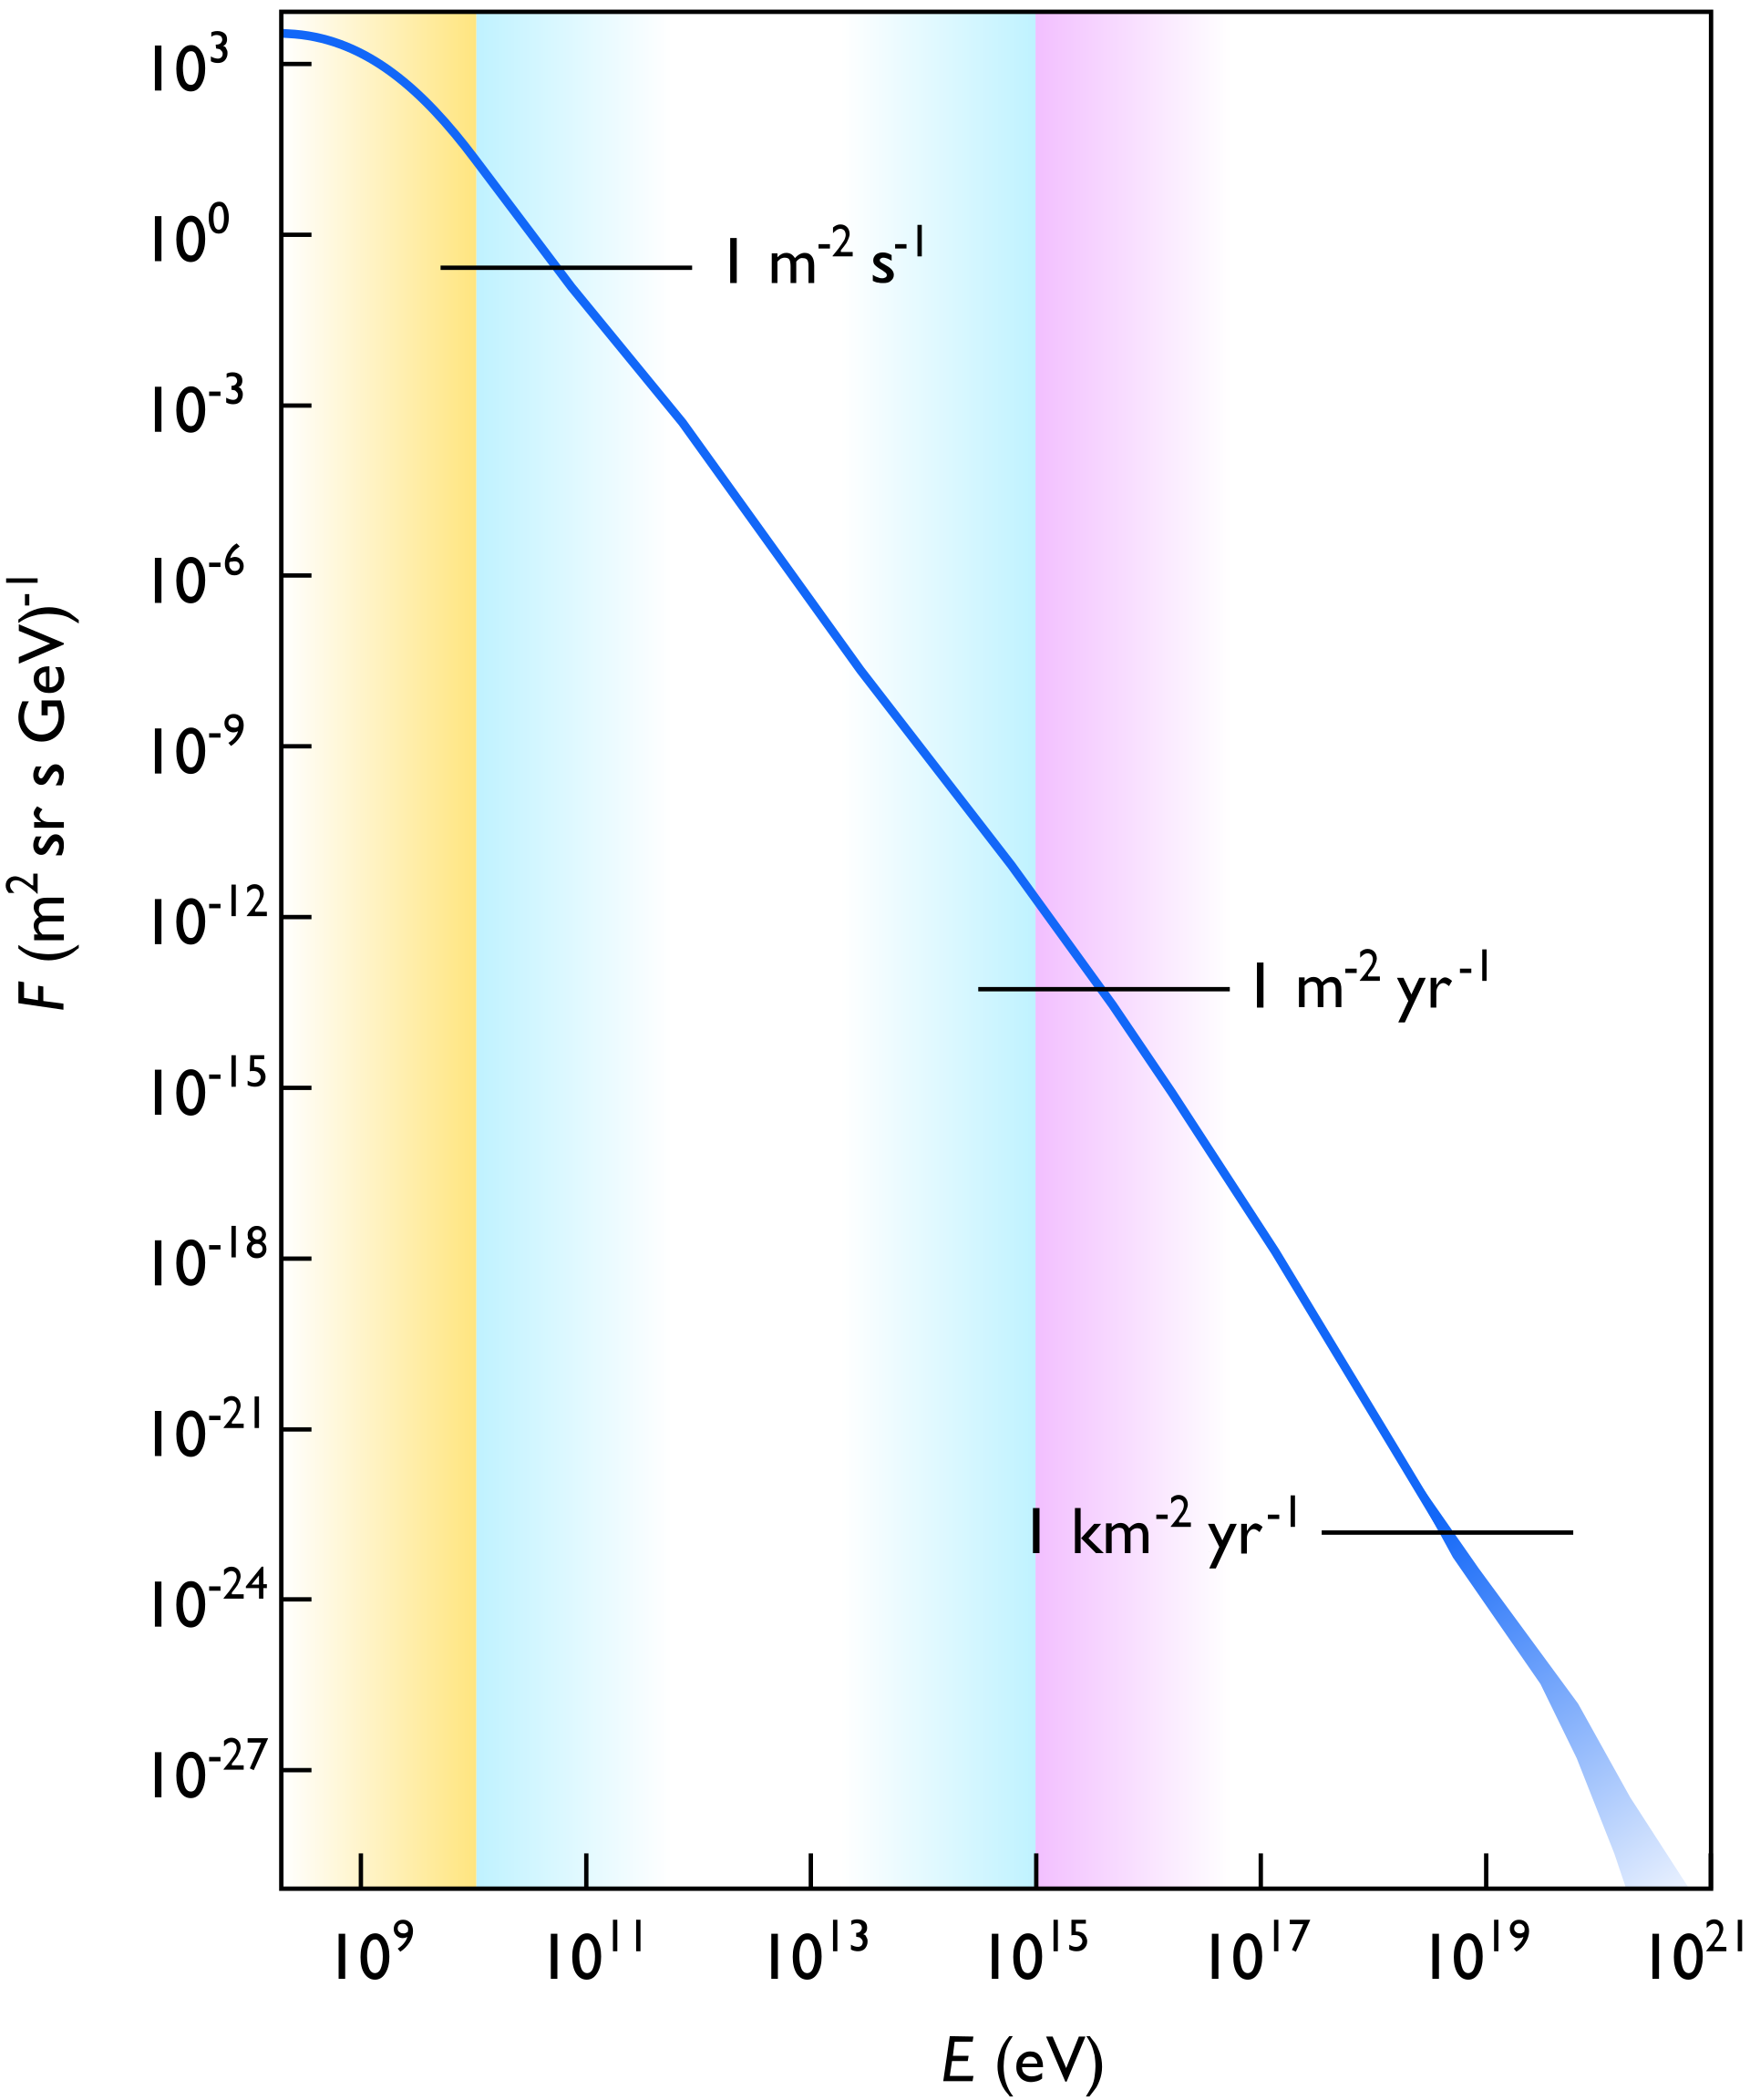
\includegraphics[width=.5\linewidth]{figs/Cosmic_ray_flux_versus_particle_energy.svg.png}
\end{figure}


\subsection*{2024年09月21日}

手元の root でグラフをトレースして表示してみようと思ったけど、Xcode の CommandLineTools がタコってて使えなかった。

\url{https://root-forum.cern.ch/t/root-on-macos-15-xcode-16/61716/8} を参考に Xcode を入れ直しているところ(2024-09-21 08:03:50)。ちゃんと動いてくれるとよいが。

一次宇宙線のグラフから傾向を読み解いてみる。
1秒1個のところは 10$^10$~eV で 10$^{-0.5}$ くらいか。
1年1個のところは 10$^{16.5}$~eV で 10$^{-13}$ と行ったところ。
強度では 12.5 桁違うことになる。一方でエネルギーでいうと 6.5 桁。
そもそも1秒と1年(31,536,000秒)で7桁違うので傾向としてはだいたいあっていることになる。
なのでエネルギーが10$^{13}$~eV のところはちょうど半分くらいなので 3.5 桁秒くらい違うところ。
10$^{14}$~eV では 4.5 桁秒に1回といったところか。1~m$^{2}$のはなしなので、10$^{4}$~m$^{2}$であれば、数秒に一回程度は降り注いでいることになる。これを使うことができればよいが。

\subsubsection*{2024-09-21 08:33:08}
 やっぱり root はコンパイルできず

\begin{codebox}{rootを Xcode MacOS15 つかってコンパイルしようとした}
   \begin{minted}[breaklines]{shell}
      While building module 'Core':
      While building module 'std' imported from input_line_1:1:
      While building module '_wctype' imported from /Applications/Xcode.app/Contents/Developer/Platforms/MacOSX.platform/Developer/SDKs/MacOSX.sdk/usr/include/wctype.h:31:
      While building module '__wctype' imported from /Applications/Xcode.app/Contents/Developer/Platforms/MacOSX.platform/Developer/SDKs/MacOSX15.0.sdk/usr/include/_wctype.h:36:
      In file included from <module-includes>:1:
      /Applications/Xcode.app/Contents/Developer/Platforms/MacOSX.platform/Developer/SDKs/MacOSX15.0.sdk/usr/include/___wctype.h:72:10: fatal error: cyclic dependency in module 'std': std -> _wctype -> __wctype -> std
      #include <ctype.h>
               ^
      /Applications/Xcode.app/Contents/Developer/Platforms/MacOSX.platform/Developer/SDKs/MacOSX15.0.sdk/usr/include/_wctype.h:36:10: fatal error: could not build module '__wctype'
      #include <_types/_wctrans_t.h>
      ~~~~~~~~^
   \end{minted}
\end{codebox}

この問題は ROOT のマイナーバージョンアップによって解決された（2024-09-29 13:39:25 追記）


\subsection*{2024年09月30日}

論文執筆のための参考文献のリストを作成する。

The virtual Muography Institute なるものが日伊の間でできている。日本の地震研究所とイタリアの火山研究所の間で結成されているとのこと。田中さんは精力的に検出器の開発の観点から仕事を進められているようである。これに乗っかっているのが東大工学部の高橋さんである。

まずポジショニングについての論文を複数読む必要が出てきている。

\subsection*{2024年10月4日}

\subsubsection*{2024-10-04 08:59:24}

シャワー面の測定がどのくらいの一次宇宙線エネルギーから可能かどうかを見積もっている。現実的な面積で可能かどうかというのが一つのポイントにはなる。測位に使えるシャワー面を同定するには、地表でのコア座標（２変数）、コア入射角度（２変数）、シャワーフロント（二次関数、３変数）が最低限必要で、あとはシャワーサイズ（１変数）や横方向分布関数などの追加情報を使うことがある。したがって少なくとも 8+2 の統計量が必要になるか。

\subsubsection*{2024-10-04 15:55:00}


100~TeV ( = $10^14$~eV) の陽子が 100~km 上空から入射したときに、どれだけのシャワー粒子が地表に到達するかのシミュレーションを行った。
全体の粒子その物の数はランダウ分布のような形をしており、3000-4000個の粒子が生成されているようである。また、エネルギーは平均 16 TeV 程度とそれ以外は光が持っていっているようである。実は光を捉えても良いのであるが、これをどう使うかは自明ではない。


\subsection*{2024年10月7日}

10, 30, 100~TeV のエネルギーについて大気シャワーのシミュレーションを行ったので、解析を進める。

saho-a:work/kpro-j2/CosmosX-0.08/Application/Example/FirstKill/fill.C 

を準備した。

10~TeV はほとんどこないことがわかっている。


\subfile{parts/diary/diary-book.tex}



\begin{qbox}

\end{qbox}

\chapter{備考}

\section{リンク}

\begin{enumerate}
   \item \href{https://docs.google.com/presentation/d/1BCVQIh1KB5iD7EcsCdXNliNvB-iTqdv0GNHVQUjJbzs/edit#slide=id.g836f55c689_0_560}{AnalysisFigure}



\end{enumerate}
\end{document}





